\documentclass[12pt,titlepage]{article}
\usepackage[spanish]{babel}
\usepackage[utf8]{inputenc}
\usepackage{amsmath}
\usepackage{amssymb}
\usepackage{graphicx}
\usepackage{caratulaMetNum}
\usepackage{float}
\usepackage{subfigure}
\usepackage{listings}
\usepackage{float}
\lstset{language=C,basicstyle=\small\tt,keywordstyle=\bf,tabsize=3,breaklines=true,linewidth=16cm,postbreak={\mbox{$\rightsquigarrow$}},prebreak={\mbox{$\rightsquigarrow$}}}

 \usepackage{a4wide}
% \usepackage{amssymb}
% \usepackage{amsmath}
 \usepackage{enumerate}
% \usepackage[utf8]{inputenc}
% \usepackage[spanish]{babel}
% \parindent = 0 pt
 \parskip = 11 pt
% \usepackage[width=15.5cm, left=3cm, top=2.5cm, height= 24.5cm]{geometry}

\usepackage{color}
\usepackage{url}
\definecolor{lnk}{rgb}{0,0,0.4}
\usepackage[colorlinks=true,linkcolor=lnk,citecolor=blue,urlcolor=blue]{hyperref}

\newcommand{\func}[2]{\texttt{#1}(#2) :}
\newcommand{\tab}{\hspace*{2em}}
\newcommand{\FOR}{\textbf{for }}
\newcommand{\TO}{\textbf{ to }}
\newcommand{\IF}{\textbf{if }}
\newcommand{\WHILE}{\textbf{while }}
\newcommand{\THEN}{\textbf{then }}
\newcommand{\ELSE}{\textbf{else }}
\newcommand{\RET}{\textbf{return }}
\newcommand{\MOD}{\textbf{ \% }}
\newcommand{\OR}{\textbf{ or }}
\newcommand{\NOT}{\textbf{ not }}
\newcommand{\tOde}[1]{\tab \small{\mathcal{O}($#1$)}}
\newcommand{\Ode}[1]{\ensuremath{\small{\mathcal{O}\left(#1\right)}}}
\newcommand{\VSP}{\vspace*{3em}}
\newcommand{\Pa}{\vspace{5mm}}
\newenvironment{pseudo}{\noindent\begin{tabular}{ll}}{\end{tabular}\VSP}

\newenvironment{while}{\WHILE \\ \setlength{\leftmargin}{0em} }{}

\newcommand{\iif}{\Leftrightarrow}
\newcommand{\gra}[1]{\noindent\includegraphics[scale=.70]{#1}\\}
\newcommand{\gras}[2]{\noindent\includegraphics[scale=#2]{#1}\\}
\newcommand{\gram}[1]{\noindent\includegraphics[scale=.50]{#1}}
\newcommand{\dirmail}[1]{\normalsize{\texttt{#1}}}
\newenvironment{usection}[1]{\newpage\begin{section}*{#1}	\addcontentsline{toc}{section}{#1}}{\end{section}}
\newenvironment{usubsection}[1]{\begin{subsection}*{#1}	\addcontentsline{toc}{subsection}{#1}}{\end{subsection}}

\newcommand{\superref}[1]{\textsuperscript{\ref{#1}}}

%\title{{\sc\normalsize Métodos Numéricos}\\{\bf Trabajo Práctico Nº1}}
%\author{\begin{tabular}{lcr}Pablo Herrero & LU & \dirmail{pablodherrero@gmail.com}\\Thomas Fischer & 489/08 & \dirmail{tfischer@dc.uba.ar}\\Kevin Allekotte & 490/08 & \dirmail{kevinalle@gmail.com} \end{tabular}}
%\date{\VSP \normalsize{Abril 2010}}
\begin{document}

\materia{Métodos Numéricos}
\titulo{Trabajo Práctico Nº3}
\subtitulo{¡El TP del Mundial!}
%\grupo{Grupo x}
\integrante{Thomas Fischer}{489/08}{tfischer@dc.uba.ar}
\integrante{Kevin Allekotte}{490/08}{kevinalle@gmail.com}
\integrante{Pablo Herrero}{332/07}{pablodherrero@gmail.com}

\abstracto{
	Tsamina mina eh eh
	Waka Waka eh eh
}

\palabraClave{Waka}
\palabraClave{Waka}
\palabraClave{eh}
\palabraClave{eh}

\begin{titlepage}
\maketitle
\end{titlepage}
\tableofcontents
\newpage

	\begin{usection}{Introducción teorica}
		El objetivo de este trabajo práctico es usar los métodos de interpolación y aproximación de funciones vistos en la materia para predecir el curso de una trayectoria.
		La trayectoria está dada por puntos en el plano en intervalos de tiempo discretos, que pueden tener errores de aproximación pero en general describen una curva suave.
		
		Los métodos que vamos a usar en este trabajo están basados en Splines y/o cuadrados mínimos.
		
		Splines es un método de interpolación. Genera una curva suave que pasa exactamente por los puntos dados.
		Esta curva está formada por muchos polinomios cúbicos que se tocan en los puntos interpolados y además los pedazos consecutivos coinciden en la derivada y en la derivada segunda.
		La variante de splines que implementamos es el Spline cúbico natural, que también cumple la propiedad de que la derivada segunda en los extremos es 0.
		
		Cuadrados mínimos es una técnica para encontrar los coeficientes de una función que aproxime a los puntos dados.
		A diferencia de splines, genera una curva suave que no necesariamente pasa por los puntos, pero los aproxima lo mejor posible.
		Por esto es más apropiado para cuando los datos no son exactos, pero la desventaja es que hay que conocer o adivinar el tipo de función.
		En el trabajo sólo vamos a usar este método para aproximar las curvas con funciones polinómicas de distintos grados.
		
		Observamos que los métodos están definidos para funciones y no para trayectorias. Podemos entonces separar nuestra trayectoria en $x(t)$ y $y(t)$ y trabajar con estas funciones.
	\end{usection}


	\begin{usection}{Desarrollo}
		Comenzamos por implementar los métodos de splines y cuadrados mínimos para poder hacer pruebas de su comportamiento para después aplicarlo a nuestro objetivo.
		Desarrollamos interfaces gráficas para ver las curvas que se estaban generando a partir de los puntos de la trayectoria.
		En la figura \ref{fig:cmspline} se observa como interpolan una secuencia de puntos los dos métodos.
		
		Vemos que cuadrados mínimos es útil para filtrar errores en los daots de entrada porque no tiene la condición de tener que pasar exactamente por los puntos.
		Genera un polinomio que aproxima muy bien a la trayectoria, siempre que se le pide el grado correcto.
		Si le pidieramos que aproxime una función con un grado demasiado bajo, no se va a ajustar correctamente y el polinomio resultante no representaría a la funcion.
		En cambio si el grado es demasiado grande, aparecerán oscilaciones inesperadas.
		
		\begin{figure}[H]
			\centering
			\subfigure{
				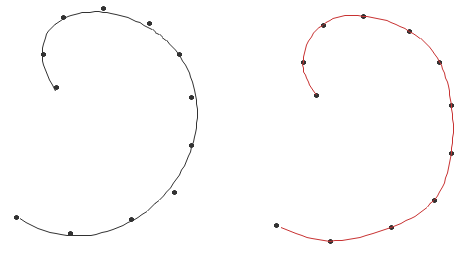
\includegraphics[scale=0.6]{img/cm_spline.png}
				%\label{fig:cm_spline1}
			}
			\subfigure{
				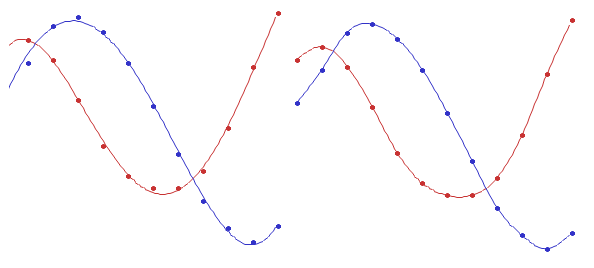
\includegraphics[scale=0.6]{img/cm_spline2.png}
				%\label{fig:cm_spline2}
			}
			\caption{
				Arriba: Interpolación de puntos de una trayectoria con cuadrados mínimos (grado 4) y splines.
				Abajo: Interpolación con cuadrados mínimos y splines de $x(t)$ y $y(t)$ de la misma trayectoria.
			}
			\label{fig:cmspline}
		\end{figure}
		
		El trabajo requería un método para predecir el curso de la trayectoria, y es por eso que nos interesa extrapolar las funciones pedidas.
		En el caso de cuadrados mínimos la extrapolación la tomamos simplemente como la continuación del polinomio para los valores más altos.
		Así, dados los puntos de una trayectoria, separamos ésta en dos funciones ($x(t)$ y $y(t)$), aplicamos cuadrados mínimos sobre cada función y obtenemos polinomios que aproximan a $x$ e $y$.
		Para estimar la trayectoria en un punto futuro $t$, simplemente evaluamos los 2 polinomios en ese $t$ y obtenemos una posición.
		
		Con Splines podemos hacer algo parecido. La diferencia es que no devuelve una función global para toda la función, sino que genera una curva formada por muchos polinomios cúbicos.
		Para extrapolar decidimos usar el último o anteúltimo polinomio de la secuencia (más detalles en discusión). Para un $t$ futuro evaluamos $SX_i$ y $SY_i$ en $t$, siendo $i=n$ ó $n-1$.
		
		En la figura \ref{fig:extrap} vemos el comportamiento de las curvas obtenidas de los métodos para tiempos futuros con la técnica recien descripta.
		Entre otras cosas, vemos que el resultado de splines es muy sensible a variaciones en las posiciones de los puntos, pero en el caso general describe mejor lo que se esperaría del futuro de la trayectoria.
		Cuadrados mínimos funciona bien cuando el grado del polinomio es aproximadamente la cantidad de curvas de la trayectoria.

		\begin{figure}[H]
			\centering
			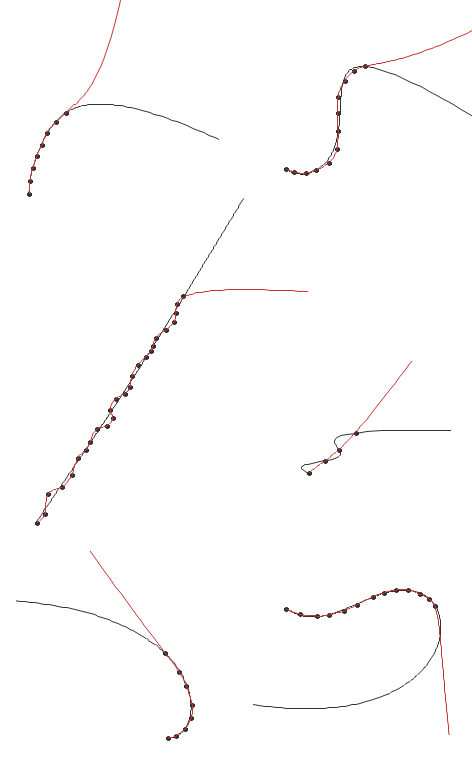
\includegraphics[scale=0.75]{img/extrap.png}
			\caption{
				Extrapolación de trayectorias con cuadrados mínimos de grado 3 o 4 (negro) y con splines (rojo).
			}
			\label{fig:extrap}
		\end{figure}
	\end{usection}
	
	En la versión final, para adivinar el futuro de la trayectoria solamente utilizamos cuadrados mínimos.
	Además definimos estrategias alternativas para cuando no disponemos de suficientes daots para extrapolar con este método.
	
	Si tenemos entre 2,3 o 4 puntos los aproximamos por un polinomio de grados 1,2,3 respectivamente y extrapolamos para calcular en que parte de la linea de gol va a llegar.
	Con más puntos primero los suavizamos. Para esto los aproximamos con un polinomio de grado a lo sumo 6 con cuadrados mínimos, y luego utilizamos para el resto del cálculo los puntos sobre esta curva con $t$ entero.
	Decidimos utilizar solamente los 6 últimos puntos del paso anterior, porque consideramos que la trayectoria anterior que realizó no nos da informacion relevante.
	A estos 6 puntos los volvemos a someter a cuadrados mínimos, esta vez de grado 2, con el objetivo de encontrar los coeficientes de la curva que está realizando.
	
	
	\begin{usection}{Resultados}
		
	\end{usection}
	
	
	\begin{usection}{Discusión}
		
	\end{usection}
	
	
	\begin{usection}{Conclusiones}
		
	\end{usection}
	
	\begin{usection}{Apéndices}
		\begin{usubsection}{Apéndice A: Enunciado}
			\begin{centering}
\bf Laboratorio de M\'etodos Num\'ericos - Primer cuatrimestre 2010 \\
\bf Trabajo Pr\'actico N\'umero 3: <El TP del Mundial! \\
\end{centering}

\vskip 25pt
\hrule
\vskip 11pt

\textbf{Introducci\'on}

Nos encontramos en la m\'axima cita del f\'utbol mundial...~de robots.
Uno de los problemas m\'as importantes a resolver en este contexto es
predecir con la mayor anticipaci\'on posible la posici\'on futura de la 
pelota en funci\'on de su posici\'on en el pasado reciente. Sobre la base
de estas predicciones se coordinan los movimientos de los jugadores de
campo y, en el caso que nos ocupa ahora, la posici\'on del arquero cuando
existe peligro de gol.

Cuando la pelota se dirige hacia nuestro arco, es muy importante que
ubiquemos el arquero en la posici\'on exacta en la que la pelota 
cruzar\'a la l\'\i nea de gol, de manera que pueda interceptarla y evitar
la ca\'\i da de nuestra valla. El sistema de control de cada equipo
suministra informaci\'on en pasos discretos. En cada paso nuestras
c\'amaras de video determinan la posici\'on de la pelota, y debemos
indicarle la acci\'on a seguir al arquero: quedarse quieto, moverse 
hacia la izquierda o moverse hacia la derecha.

Los postes del arco est\'an ubicados en las coordenadas (-1,0) y (1,0),
y la l\'\i nea de gol es el segmento entre estos dos puntos. Se marca
un gol cuando la pelota cruza este segmento. Vistos desde arriba, la pelota
es un c\'\i rculo de 0.10 de radio y el arquero 
se representa mediante un segmento paralelo a la l\'\i nea de gol de 0.10 
de longitud y ubicado sobre la misma.
% es un jugador cuadrado de 0.10 de lado, 
% cuyo punto central est\'a ubicado sobre la l\'\i nea de gol. 
Inicialmente el punto central del arquero se encuentra en la
posici\'on (0,0), y en cada paso se le indica al arquero qu\'e acci\'on
debe tomar. Si se le indica un movimiento hacia alguno de los lados
(izquierda o derecha) y en el paso anterior estaba quieto o se estaba
moviendo hacia ese mismo lado, entonces el arquero se mueve 0.05 en
la direcci\'on indicada. Por el contrario, si en el paso anterior se
hab\'\i a indicado un movimiento en la direcci\'on opuesta, entonces
el arquero se queda quieto durante el paso actual.

Un problema fundamental que debe enfrentarse es la presencia de ruido
en las mediciones de la posici\'on de la pelota. El sistema de visi\'on
est\'a sujeto a vibraciones, golpes y errores de captura de datos,
que hacen que las mediciones de la pelota sufran errores, e incluso 
registren posiciones irreales (es un efecto muy com\'un que la pelota
``desaparezca'' en un cuadro y vuelva a aparecer en el cuadro siguiente).
Por otra parte, la pelota no siempre viaja hacia el arco en l\'\i nea
recta sino que puede describir curvas m\'as o menos complicadas,
dependiendo del ``efecto'' dado por el jugador al momento de impactar
la pelota y de posibles curvaturas en la superficie del campo de juego.

\textbf{Enunciado}

El objetivo del trabajo pr\'actico es implementar un programa que
tome como datos las posiciones sucesivas de la pelota y que determine
en cada paso qu\'e debe hacer el arquero para evitar el gol. Se deben
tomar las mediciones con la posici\'on de la pelota de un archivo
de entrada, que tiene en cada l\'inea el n\'umero de medici\'on,
la posici\'on $x$ y la posici\'on $y$ de la pelota, separados
por espacios. La \'ultima l\'\i nea del archivo tiene -1 como
primer dato, indicando el fin de las mediciones.

En cada paso, el programa debe determinar qu\'e acci\'on debe tomar
el arquero, escribiendo la decisi\'on correspondiente en un archivo
de salida. Cada l\'\i nea de este archivo debe tener el n\'umero
de medici\'on y la acci\'on del arquero (0: quedarse quieto, 1: izquierda,
2: derecha), separados por espacio. El programa debe tomar por
l\'\i nea de comandos el nombre del archivo de entrada y el nombre
del archivo de salida. Dado que estamos simulando
la decisi\'on en tiempo real, para generar la acci\'on correspondiente
a una medici\'on el programa solamente puede usar la informaci\'on
de esa medici\'on y las anteriores (es decir, no se puede consultar
lo que suceder\'a en el futuro para tomar las decisiones).

Las instrucciones al arquero deben estar basadas en un mecanismo de
predicci\'on de la posici\'on futura de la pelota. Esta predicci\'on
se debe realizar sobre la base de alg\'un m\'etodo num\'erico visto
en la materia, o alguna variaci\'on de los temas vistos en clase.
Sugerimos consultar con los docentes del laboratorio para validar
los enfoques que propongan implementar.

Se adjunta a este enunciado un programa simulador de los tiros al
arco, junto con algunos archivos de prueba para testear el formato
de los archivos de entrada y salida. Todos los programas participar\'an
de un campeonato mundial de arqueros, y el grupo cuyo arquero logre
atajar la mayor cantidad de tiros al arco se har\'a acreedor a la
copa ``Laboratorio de M\'etodos Num\'ericos'' al mejor guardavallas del
mundial.

\textbf{Preguntas adicionales}

\begin{enumerate}
\item >En qu\'e minuto del partido Argentina-Uni\'on Sovi\'etica del mundial
Italia '90 se lesion\'o Nery Pumpido, arquero de la selecci\'on
argentina?

\item >C\'omo se llamaba el \'arbitro del partido Argentina-Francia en
el mundial Argentina '78?

\item >Cu\'antos jugadores fueron expulsados en el mundial Italia '90
por derribar a Claudio Paul Caniggia?

\item >Cu\'antos pases hizo la selecci\'on argentina antes del gol de Maradona
ante Grecia en el mundial EEUU 94?

\item >Cu\'antos minutos jug\'o Ricardo Bochini en la semifinal del
mundial M\'exico '86?

\item >C\'omo se llamaba el arquero suplente de la selecci\'on argentina
en la final del mundial Uruguay '30?
\end{enumerate}

\vskip 15pt

\hrule

\vskip 11pt

Fecha de entrega: Viernes 25 de Junio

		\end{usubsection}
		
		\newpage
		\begin{usubsection}{Apéndice B: Codigos Fuente}
			
		\end{usubsection}
	\end{usection}
	
	
	\begin{usection}{Referencias}
	\begin{enumerate}
		\item \label{ref:spline} \texttt{http://en.wikipedia.org/wiki/Spline\_(mathematics)} \\ Artículo de wikipedia sobre splines con un pseudocódigo de la implementación de Spline cúbico natural.
		\item \label{ref:waka} \texttt{http://waka-waka} \\ Waka Waka
	\end{enumerate}	
	\end{usection}

\end{document}

